% pdflatex Homework9.tex; evince Homework9.pdf & 


\documentclass[12pt,pdftex]{article}
\usepackage{amsmath,amsthm,setspace,graphicx,natbib,color,xfrac,amssymb,graphicx}

\usepackage[inline]{enumitem}

\textwidth 7.0 truein
\oddsidemargin -0.25in   %left-hand edge
\evensidemargin -0.5 truein  %right-hand edge
\topmargin -0.85in      %top of paper to top of head, pulls whole unit
\textheight 9.5in


\begin{document}

\begin{center}
\textbf{Math 2270-001 \hspace{10pt} Linear Algebra \hspace{10pt}  Fall 2016}
\end{center}

\hfill Tanner Kvarfordt

\hfill Math 2270

\hfill Assignment \#9


\begin{itemize}
\item[5.3.1)] Solve these linear equations by Cramer's Rule $x_j=\frac{|B_j|}{|A|}$: \\ \vspace{4mm}
\begin{enumerate*}
\item[a)] $\begin{array}{ccc} 
			2x_1+5x_2 & = & 1 \\ 
            x_1+4x_2& = & 2
          \end{array}$ \hspace{20mm}
\item[b)] $\begin{array}{lllll} 
			2x_1 + \hspace{2mm}x_2 & = & 1 \\
            \hspace{2mm}x_1+2x_2+\hspace{2mm}x_3 & = & 0 \\
            \hspace{13mm}x_2+2x_3 & = & 0
          \end{array}$
\end{enumerate*}

\textit{Solution.}
\begin{itemize}
\item[a)] $A=\begin{bmatrix}
		  2 & 5 \\ 1 & 4
		  \end{bmatrix}$, 
          $B_1=\begin{bmatrix}
          1 & 5 \\ 2 & 4
          \end{bmatrix}$, 
          $B_2=\begin{bmatrix}
          2 & 1 \\ 1 & 2
          \end{bmatrix}$ \\ $\Rightarrow
          |A|=8-5=3$, $|B_1|=4-10=-6$, $|B_2|=4-1=3$ \\ $\Rightarrow
          x_1=\frac{|B_1|}{|A|}=\frac{-6}{3}=-2$, and $x_2=\frac{|B_2|}{|A|}=\frac{3}{3}=1$
          
\item[b)] $A=\begin{bmatrix}
		  2 & 1 & 0 \\ 1 & 2 & 1 \\ 0 & 1 & 2
		  \end{bmatrix}$, 
          $B_1=\begin{bmatrix}
          1 & 0 & 0 \\ 1 & 2 & 1 \\ 0 & 1 & 2
          \end{bmatrix}$, 
          $B_2=\begin{bmatrix}
		  2 & 1 & 0 \\ 1 & 0 & 0 \\ 0 & 1 & 2
		  \end{bmatrix}$, 
          $B_3=\begin{bmatrix}
		  2 & 1 & 0 \\ 1 & 2 & 1 \\ 1 & 0 & 0
		  \end{bmatrix}$ \\ $\Rightarrow 
          |A|=(-1)^{3+2}\left|\begin{matrix}
          2 & 0 \\ 1 & 1
          \end{matrix}\right| +
          (-1)^{3+3}2\left|\begin{matrix}
          2 & 1 \\ 1 & 2
          \end{matrix}\right|=-2+2(4-1)=4$, \\ $
          |B_1|=(-1)^{1+1}\left|\begin{matrix}
          2 & 1 \\ 1 & 2
          \end{matrix}\right| = 4 - 1 = 3$, \\ $
          |B_2|=(-1)^{3+3}2\left|\begin{matrix}
          2 & 1 \\ 1 & 0
          \end{matrix}\right|=2(-1)=-2$, \\ $
          |B_3|=(-1)^{3+2}\left|\begin{matrix}
          2 & 1 \\ 1 & 0
          \end{matrix}\right|=(-1)(-1)=1$ \\ $\Rightarrow 
          x_1=\frac{|B_1|}{|A|}=\frac{3}{4}$, $x_2=\frac{|B_2|}{|A|}=\frac{-1}{2}$, and $x_3=\frac{|B_3|}{|A|}=\frac{1}{4}$
\end{itemize}

\item[5.3.16)] \begin{itemize}
\item[a)] Find the area of the parallelogram with edges $\vec{v}=(3,2)$ and $\vec{w}=(1,4)$.
\item[b)] Find the area of the triangle with sides $\vec{v}$, $\vec{w}$, and $\vec{v}+\vec{w}$. Draw it.
\item[c)] Find the area of the triangle with sides $\vec{v}$, $\vec{w}$, and $\vec{w}-\vec{v}$. Draw it.
\end{itemize}

\textit{Solution.}
\begin{itemize}
\item[a)] Area = abs$\left(\left|\begin{matrix} 3 & 1 \\ 2 & 4\end{matrix}\right|\right)=$ abs$(12-2)=10$

\item[b)] Area = abs$\left(\frac{1}{2}\left|\begin{matrix} 3 & 1 \\ 2 & 4\end{matrix}\right|\right)=$ abs$(\frac{1}{2}(12-2))=5$ \\ \begin{center}
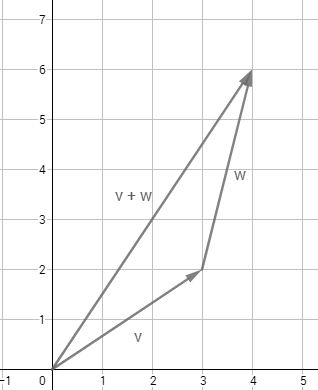
\includegraphics[scale=0.52333]{triangle1.JPG}
\end{center}

\item[c)] By the same logic as in part (b), the area equals $5$. \\ \begin{center}
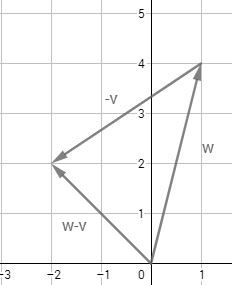
\includegraphics[scale=0.8]{triangle2.JPG}
\end{center}
\end{itemize}

\item[6.1.2)] Find the eigenvalues and the eigenvectors of these two matrices:
\[A=\begin{bmatrix}1 & 4 \\ 2 & 3\end{bmatrix} \text{ and } B=A+I=\begin{bmatrix}2 & 4 \\ 2 & 4\end{bmatrix}\]
$A+I$ has the $\rule{1cm}{0.15mm}$ eigenvectors as $A$. Its eigenvalues are $\rule{1cm}{0.15mm}$ by 1.

\textit{Solution.}
\begin{itemize}
\item[a)] \begin{itemize}
		     \item[i)] $|A-\lambda I|=\left|\begin{matrix}
		     			1-\lambda & 4 \\ 2 & 3-\lambda
		     		    \end{matrix}\right|=0 \Rightarrow 3-4\lambda+\lambda^2-8=\lambda^2-4\lambda-5=0$ \\$
                        \Rightarrow (\lambda-5)(\lambda+1)=0 \Rightarrow \lambda_5=5, \lambda_{-1}=-1$
                        
             \item[ii)] $(A-\lambda_{-1}I)\vec{x}=\vec{0} \Rightarrow 
             			 \begin{bmatrix}2 & 4 \\ 2 & 4 \end{bmatrix}\vec{x}=\vec{0} \longrightarrow 
                         \begin{bmatrix}2 & 4 \\ 0 & 0 \end{bmatrix}\vec{x}=\vec{0}$.  
                         Let our free variable, $x_2=1$ 
                         and solve to get $x_1=-2 \Rightarrow \vec{v}_{-1}=\begin{bmatrix}-2 \\ 1 \end{bmatrix}$. \\
                         $(A-\lambda_{5}I)\vec{x}=\vec{0} \Rightarrow 
                         \begin{bmatrix}-4 & 4 \\ 2 & -2 \end{bmatrix}\vec{x}=\vec{0}
                         \longrightarrow \begin{bmatrix}-4 & 4 \\ 0 & 0 \end{bmatrix}\vec{x}=\vec{0}$. 
                         $x_2$ is a free variable, $x_1$ is a pivot variable. Let $x_2=1$ and solve to get $x_1=1$.
                         Therefore $\vec{v_5}=\begin{bmatrix}1 \\ 1\end{bmatrix}$.
             
	      \end{itemize}
\item[b)] \begin{itemize}
		     \item[i)] $|B-\lambda I|=\left|\begin{matrix}
		     			2-\lambda & 4 \\ 2 & 4-\lambda
		     		    \end{matrix}\right|=0 \Rightarrow 8-6\lambda+\lambda^2-8=\lambda^2-6\lambda=0$ \\$
                        \Rightarrow \lambda(\lambda-6)=0 \Rightarrow \lambda_0=0, \lambda_6=6$
             \item[ii)] $(B-\lambda_0I)\vec{x}=\vec{0} \Rightarrow 
             			B\vec{x}=\vec{0} \longrightarrow \begin{bmatrix}
             			2 & 4 \\ 0 & 0
             			\end{bmatrix}\vec{x}=\vec{0}$. Let our free variable, $x_2=1$ and solve to get $x_1=-2$.
                        Therefore $\vec{v_0}=\begin{bmatrix}-2 \\ 1\end{bmatrix}$. \\
                        
                        $(B-\lambda_6I)\vec{x}=\vec{0} \Rightarrow 
             			\begin{bmatrix}-4 & 4 \\ 2 & -2\end{bmatrix}\vec{x}=\vec{0} \longrightarrow \begin{bmatrix}
             			-4 & 4 \\ 0 & 0
             			\end{bmatrix}\vec{x}=\vec{0}$. Let our free variable, $x_2=1$ and solve to get $x_1=1$.
                        Therefore $\vec{v_6}=\begin{bmatrix}1 \\ 1\end{bmatrix}$.
                        
           \item[c)] $A+I$ has the same eigenvectors as $A$. Its eigenvalues are increased by 1.
	      \end{itemize}
\end{itemize}

\item[6.1.4)] Compute the eigenvalues and eigenvectors of $A$ and $A^2$:
\[A=\begin{bmatrix}-1 & 3 \\ 2 & 0\end{bmatrix} \text{ and } A^2=\begin{bmatrix}7 & -3 \\ -2 & 6\end{bmatrix}\]
$A^2$ has the same $\rule{1cm}{0.15mm}$ as $A$. When $A$ has eigenvalues $\lambda_1$ and $\lambda_2$, $A^2$ has eigenvalues $\rule{1cm}{0.15mm}$. In this example, why is $\lambda_1^2+\lambda_2^2=13$?

\textit{Solution.}
\begin{itemize}
\item[a)] \begin{itemize}
		     \item[i)] $|A-\lambda I|=\left|\begin{matrix}
		     			-1-\lambda & 3 \\ 2 & -\lambda
		     			\end{matrix}\right|=\lambda^2+\lambda-6=(\lambda+3)(\lambda-2)=0
                        \Rightarrow \lambda_{-3}=-3$, $\lambda_2=2$
             \item[ii)] $(A-\lambda_{-3}I)\vec{x}=\vec{0} \Rightarrow 
             			\begin{bmatrix}
             			2 & 3 \\ 2 & 3
             			\end{bmatrix}\vec{x}=\vec{0} \longrightarrow 
                        \begin{bmatrix}
                        2 & 3 \\ 0 & 0
                        \end{bmatrix}\vec{x}=\vec{0}$. Free var: $x_2=1$, so \\$\vec{v}_{-3}=(\frac{-3}{2},1)$. \\
                        $(A-\lambda_2I)\vec{x}=\vec{0} \Rightarrow 
             			\begin{bmatrix}
             			-3 & 3 \\ 2 & -2
             			\end{bmatrix}\vec{x}=\vec{0} \longrightarrow 
                        \begin{bmatrix}
                        -3 & 3 \\ 0 & 0
                        \end{bmatrix}\vec{x}=\vec{0}$. Free var: $x_2=1$, so $\vec{v}_{2}=(1,1)$.
	      \end{itemize}
\item[b)] \begin{itemize}
		     \item[i)] $|A^2-\lambda I|=\left|\begin{matrix}
		     			7-\lambda & -3 \\ -2 & 6-\lambda
		     			\end{matrix}\right|=\lambda^2-13\lambda+36=(\lambda-9)(\lambda-4)=0
                        \Rightarrow \lambda_{9}=9$, $\lambda_4=4$
             \item[ii)] $(A^2-\lambda_9I)\vec{x}=\vec{0} \Rightarrow 
             			\begin{bmatrix}
             			-2 & -3 \\ -2 & -3
             			\end{bmatrix}\vec{x}=\vec{0} \longrightarrow 
                        \begin{bmatrix}
                        -2 & -3 \\ 0 & 0
                        \end{bmatrix}\vec{x}=\vec{0}$. Free var: $x_2=1$, so $\vec{v}_9=(\frac{-3}{2},1)$. \\
                        $(A^2-\lambda_4I)\vec{x}=\vec{0} \Rightarrow 
             			\begin{bmatrix}
             			3 & -3 \\ -2 & 2
             			\end{bmatrix}\vec{x}=\vec{0} \longrightarrow 
                        \begin{bmatrix}
                        3 & -3 \\ 0 & 0
                        \end{bmatrix}\vec{x}=\vec{0}$. Free var: $x_2=1$, so $\vec{v}_4=(1,1)$.
	      \end{itemize}
\item[c)] eigenvectors
\item[d)] $\lambda_1^2$ and $\lambda_2^2$
\item[e)] Because $\lambda_1=-3$ and $\lambda_2=2$, and $9+4=13$.
\end{itemize}


\item[6.1.9)] What do you do to the equation $A\vec{x}\lambda\vec{x}$, in order to prove (a), (b), and (c)?
\begin{itemize}
\item[a)] $\lambda^2$ is an eigenvalue of $A^2$, as in Problem 4 (See Textbook).
\item[b)] $\lambda^{-1}$ is an eigenvalue of $A^{-1}$, as in Problem 3 (See Textbook).
\item[c)] $\lambda+1$ is an eigenvalue of $A+I$, as in Problem 2 (See Textbook).
\end{itemize}

\textit{Solution.}
\begin{itemize}
\item[a)] $A^2\vec{x}=\lambda^2\vec{x}$
\item[b)] $A^{-1}\vec{x}=\frac{1}{\lambda}\vec{x}$
\item[c)] $(A+I)\vec{x}=(\lambda + 1)\vec{x}$
\end{itemize}

\end{itemize}

\noindent Problem S1: Assume the 3x3 matrix $\mathbf{A}$ has eigenvalues 0, 2, 6 with linearly independent eigenvectors $\vec{v}_0$, $\vec{v}_2$, and $\vec{v}_6$ (the subscript for each eigenvector is the corresponding eigenvalue). 
\begin{itemize}
\item[(a)] Compute the trace and determinant of $\mathbf{A}$.
\item[(b)] What is a basis for $\mathcal{N}(\mathbf{A})$?  What is a basis for $\mathcal{C}(\mathbf{A})$?
\item[(c)] Find a particular solution to $\mathbf{A}\vec{x} = \vec{v}_2+\vec{v}_6$.  What is the complete solution to $\mathbf{A}\vec{x} = \vec{v}_2+\vec{v}_6$?
\item[(d)] $\mathbf{A}\vec{x}=\vec{v}_0$ does not have a solution.  If it did then \underline{\hspace{50pt}} would be in $\mathcal{C}(\mathbf{A})$.  But this is not possible because ...? (Hint: Think about dimensions.)
\end{itemize}

\textit{Solution.}
\begin{itemize}
\item[a)] tr$(A)=0+2+6=8$ and $|A|=0\cdot2\cdot6=0$
\item[b)] $\mathcal{N}(\mathbf{A})=\mathcal{N}(\mathbf{A}-\lambda_0I)$, so $\{\vec{v_0}\}$ is a basis of $
		  \mathcal{N}(\mathbf{A})$. The linearly independent column vectors of $A$ form a basis of $\mathcal{C}(\mathbf{A})$.
          $\vec{v}_2$ and $\vec{v}_6$ also form a basis of $\mathcal{C}(\mathbf{A})$.
\item[c)] How tho?
\item[d)] If it had a solution, $\vec{v}_0$ would be in $\mathcal{C}(\mathbf{A})$. This is impossible because dim$[\mathcal{C}(\mathbf{A})]=2$ and $\vec{v}_2$ and $\vec{v}_6$ are the basis of $\mathcal{C}(\mathbf{A})$.
\end{itemize}

\noindent Problem S2: Complete the following:
\begin{itemize}
\item[(a)] If $\mathbf{A}$ is singular, then $\det(\mathbf{A}) =$ \underline{\hspace{30pt}}
\item[(b)] If $\mathbf{A}$ is invertible, then $\det(\mathbf{A})$ is \underline{\hspace{30pt}}
\item[(c)] If $\mathbf{A}$ is (upper or lower) triangular, then $\det(\mathbf{A}) =$ \underline{\hspace{30pt}}
\item[(d)] The determinant of the identity matrix $\mathbf{I}$ is $|\mathbf{I}| =$ \underline{\hspace{30pt}}
\item[(e)] If $\mathbf{A}$ has an inverse, then $\det(\mathbf{A}^{-1}) =$ \underline{\hspace{30pt}}
\end{itemize}

\textit{Solution.}
\begin{itemize}
\item[a)] $|A|=0$
\item[b)] $|A|\neq0$
\item[c)] $|A|=$ The product of $A$'s diagonal entries
\item[d)] $|I|=1$
\item[e)] $|A^{-1}|=\frac{1}{|A|}$
\end{itemize}

\noindent Problem S3:  Assume $\mathbf{A}$ is a 4x4 matrix with eigenvalues 0,1,-1,2.
\begin{itemize}
\item[(a)] What is the rank of $\mathbf{A}$?
\item[(b)] What is the determinant of $\mathbf{A}^\text{T}\mathbf{A}$?
\item[(c)] What is the determinant of $\mathbf{A}\mathbf{A}^\text{T}$?
\item[(d)] What is the dimension of $\mathcal{C}(A)$? 
\item[(e)] What is the dimension of $\mathcal{N}(A)$?
\item[(f)] How many solutions are there to $\mathbf{A}\vec{x}=\vec{b}$? 
\end{itemize}

\textit{Solution.}
\begin{itemize}
\item[a)] r$(A)=3$
\item[b)] Since we have $0$ as an eigenvalue, $|A|=0$ and therefore $|A^TA|=|A^T||A|=0$.
\item[c)] Since we have $0$ as an eigenvalue, $|A|=0$ and therefore $|AA^T|=|A||A^T|=0$.
\item[d)] dim$[C(A)]=$ r$(A)=3$
\item[e)] dim$[N(A)]=n-$ r$(A)=1$
\item[f)] Since $A$ has neither full column nor full row rank, there are either $0$ or infinite solutions to $\mathbf{A}\vec{x}=\vec{b}$.
\end{itemize}

\end{document}


$\vec{u}=\left[\begin{array}{c} 1 \\ 0\end{array}\right]$

$\left[\begin{array}{cc}  & \\  & \end{array}\right]$

$\left[\begin{array}{ccc}  &  & \\  &  & \\ & & \end{array}\right]$
